\documentclass[11pt,a4paper]{article}

\usepackage{iftex}
\ifPDFTeX
  \usepackage[T1]{fontenc}
  \usepackage[utf8]{inputenc}
\else
  \usepackage{fontspec}
  \defaultfontfeatures{Ligatures=TeX}
  \setmainfont{DejaVu Serif}
  \setsansfont{DejaVu Sans}
  \setmonofont{DejaVu Sans Mono}
\fi
\usepackage[english]{babel}
\usepackage{amsmath,amssymb,bm}
\usepackage{array}
\usepackage{booktabs}
\usepackage{enumitem}
\usepackage{geometry}
\usepackage{graphicx}
\usepackage{hyperref}
\usepackage{siunitx}
\usepackage{xcolor}

\geometry{margin=23mm}
\hypersetup{colorlinks=true,linkcolor=blue!55!black,urlcolor=blue!55!black}
\sisetup{per-mode=symbol}

\newcommand{\vect}[1]{\bm{#1}}
\newcommand{\dd}{\mathrm{d}}
\newcommand{\FL}{\mathrm{FL}}
\newcommand{\FR}{\mathrm{FR}}
\newcommand{\RL}{\mathrm{RL}}
\newcommand{\RR}{\mathrm{RR}}

\title{Controllers and Torque Allocators\\AGH Racing DV Control}
\author{FS AGH Racing Driverless}
\date{\today}

\begin{document}
\maketitle
\tableofcontents

\begin{figure}[p]
\centering
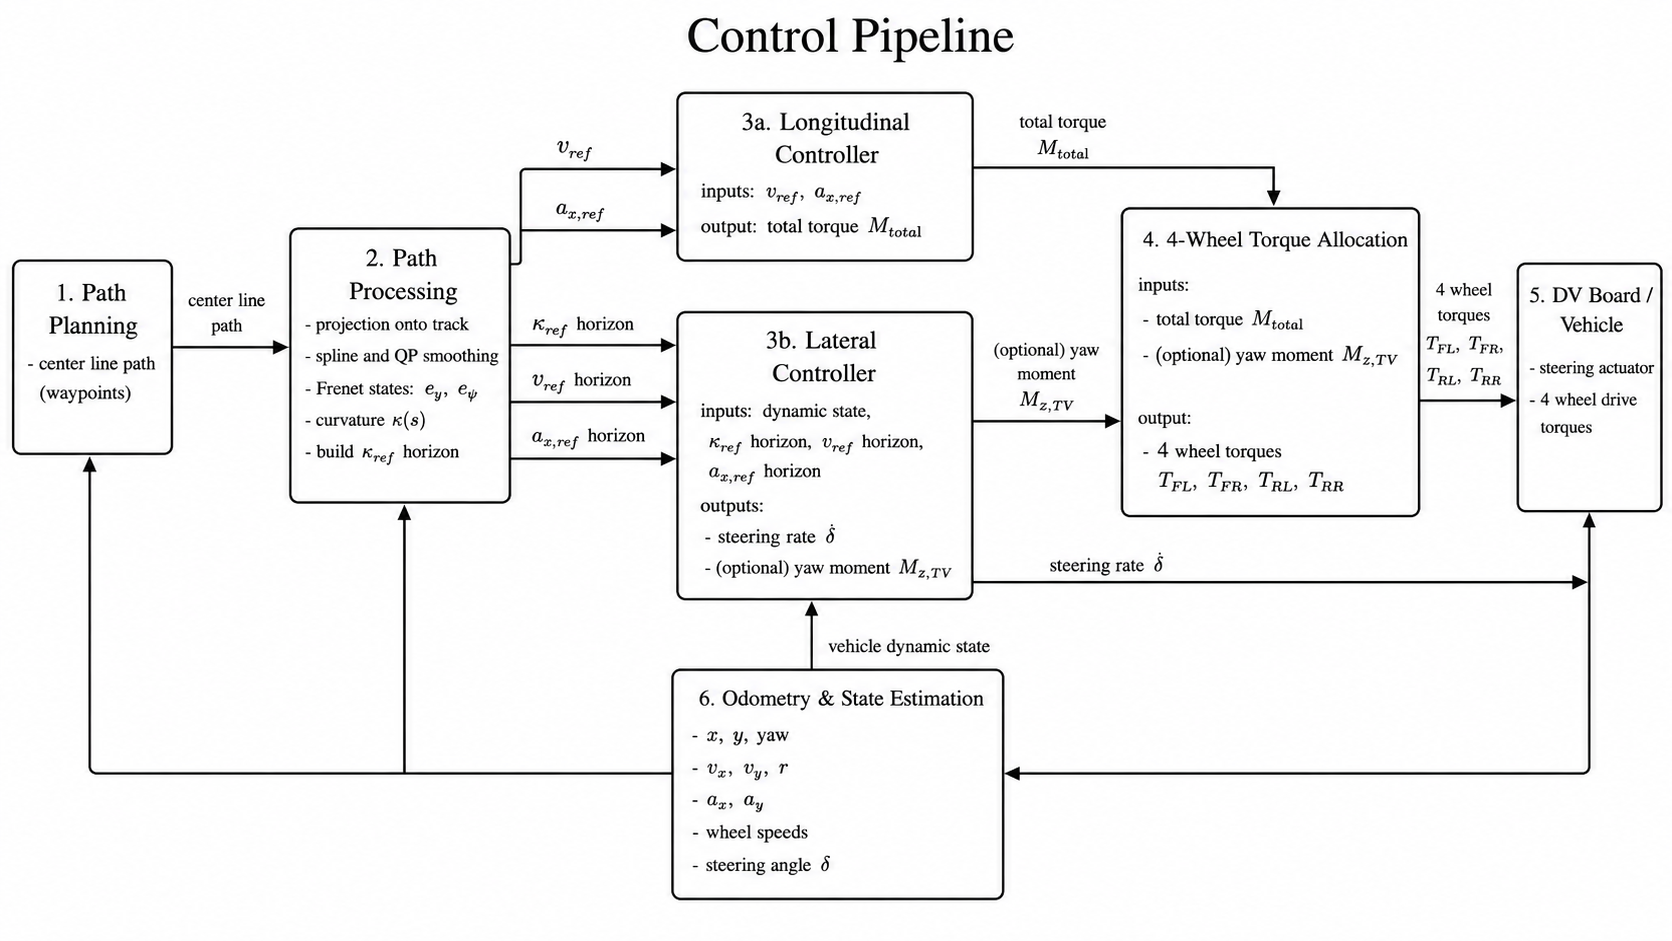
\includegraphics[width=\textwidth]{control_pipeline.png}
\caption{Control pipeline}
\label{fig:control-pipeline}
\end{figure}

\section{Scope and conventions}

This document describes the shared implementation used by the packages:
\begin{itemize}[nosep]
  \item \texttt{dv\_control},
  \item \texttt{dv\_skidpad\_control},
  \item \texttt{dv\_acc\_launch\_control}.
\end{itemize}
All three packages use the same unbounded LTV MPC for lateral control.
In \texttt{dv\_control}, the longitudinal reference is generated by the
forward--backward (BF) profile.

The body-fixed convention is $x$ forward, $y$ left, and positive yaw
counter-clockwise. Positive $a_y$ is acceleration to the left and therefore
loads the right-hand wheels. Positive $a_x$ loads the rear axle. Wheel torque
is expressed in \si{\newton\metre}; positive torque drives the vehicle.

\begin{table}[htbp]
\centering
\begin{tabular}{lll}
\toprule
Symbol & Unit & Meaning\\
\midrule
$e_y,e_\psi$ & \si{\metre}, \si{\radian} & Frenet and heading errors\\
$v_x,v_y,r$ & \si{\metre\per\second}, \si{\metre\per\second},
  \si{\radian\per\second} & body velocities and yaw rate\\
$\delta,\dot\delta,\delta_{\rm cmd}$ & \si{\radian},
  \si{\radian\per\second}, \si{\radian} & steering-system state\\
$M_{z,\rm TV}$ & \si{\newton\metre} & torque-vectoring yaw-moment request\\
$l_f,l_r,L$ & \si{\metre} & CG-to-axle distances, $L=l_f+l_r$\\
$t_f,t_r$ & \si{\metre} & front and rear track widths\\
\bottomrule
\end{tabular}
\end{table}

\section{Path processing and BF profile}

The path is smoothed and parameterized by arc length $s$. Projecting the
vehicle onto the spline gives $e_y$, $e_\psi$, and curvature $\kappa(s)$.
The local speed limit imposed by lateral acceleration is
\begin{equation}
 v_\kappa(s)=
 \min\left(v_{\max},
 \sqrt{\frac{a_{y,\max}}{\max(|\kappa(s)|,\varepsilon)}}\right).
\end{equation}

Lateral acceleration consumes part of the available tire friction. The
longitudinal-acceleration limit is
\begin{align}
 a_y &= v^2|\kappa|,\\
 a_{x,\rm ell} &=
 a_{x,\max}\sqrt{\max\left(0,1-
 \left(\frac{a_y}{a_{y,\max}}\right)^2\right)}.
\end{align}
The power limit and resistance forces give
\begin{align}
 F_{\rm res}(v)&=C_dv^2+C_{rr}mg,\\
 a_{x,\rm drive}&=\min\left(a_{x,\rm ell},
 \max\left(0,\frac{P_{\rm drive}/\max(|v|,v_\varepsilon)
 -F_{\rm res}}{m}\right)\right),\\
 a_{x,\rm brake}&=\min\left(a_{x,\rm ell},
 \max\left(0,\frac{P_{\rm brake}/\max(|v|,v_\varepsilon)
 +F_{\rm res}}{m}\right)\right).
\end{align}

For a spatial step $\Delta s$, the forward pass limits the reachable speed:
\begin{equation}
 v_{i+1}\leftarrow\min\left(v_{i+1},
 \sqrt{v_i^2+2a_{x,\rm drive,i}\Delta s}\right),
\end{equation}
and the backward pass guarantees that the vehicle can brake before a future
constraint:
\begin{equation}
 v_i\leftarrow\min\left(v_i,
 \sqrt{v_{i+1}^2+2a_{x,\rm brake,i}\Delta s}\right).
\end{equation}
The acceleration reference is computed without time differentiation:
\begin{equation}
 a_{x,\rm ref,i}=\frac{v_{i+1}^2-v_i^2}{2\Delta s}.
\end{equation}

The feedforward torque includes wheel rotational inertia:
\begin{align}
 m_{\rm eq}&=m+n_w\frac{I_w}{R_w^2},\\
 M_{\rm total,ff}&=m_{\rm eq}a_{x,\rm ref}R_w+M_{\rm res}(v_x).
\end{align}

\section{Shared unbounded LTV MPC}

\subsection{State and input}

The optimizer state and input are
\begin{align}
\vect{x}&=
\begin{bmatrix}
e_y&e_\psi&v_y&r&\delta&\dot\delta&\delta_{\rm cmd}&M_{z,\rm TV}
\end{bmatrix}^{\!T},\\
\vect{u}&=
\begin{bmatrix}
\dot\delta_{\rm cmd}&\dot M_{z,\rm TV}
\end{bmatrix}^{\!T}.
\end{align}
No additional states are introduced between the command and the actuator
model.

\subsection{Nonlinear model used for linearization}

The Frenet kinematics are
\begin{align}
\dot s &=
\frac{v_x\cos e_\psi-v_y\sin e_\psi}{1-\kappa e_y},\\
\dot e_y&=v_x\sin e_\psi+v_y\cos e_\psi,\\
\dot e_\psi&=r-\kappa\dot s.
\end{align}
The velocity used in denominators is lower-bounded by $v_{\min}$ to avoid a
numerical singularity.

The bicycle-model slip angles are
\begin{align}
\alpha_f&=\delta-\operatorname{atan2}(v_y+l_fr,v_x),\\
\alpha_r&=-\operatorname{atan2}(v_y-l_rr,v_x).
\end{align}
The tire model is a simplified Magic Formula:
\begin{align}
F_{y,f}&=F_{z,f}D_f\sin\!\left(C_f\arctan(B_f\alpha_f)\right),\\
F_{y,r}&=F_{z,r}D_r\sin\!\left(C_r\arctan(B_r\alpha_r)\right).
\end{align}
The lateral dynamics are
\begin{align}
\dot v_y&=\frac{F_{y,f}+F_{y,r}}{m}-v_xr,\\
\dot r&=\frac{l_fF_{y,f}-l_rF_{y,r}+M_{z,\rm TV}}{I_z}.
\end{align}

The steering actuator is a second-order PT2 element. With
$\nu_\delta\equiv \dd\delta/\dd t$:
\begin{align}
\dot\delta&=\nu_\delta,\\
\dot\nu_\delta&=-\omega_s^2\delta
-2\zeta_s\omega_s\nu_\delta+\omega_s^2\delta_{\rm cmd},\\
\dot\delta_{\rm cmd}&=u_\delta,\qquad
\dot M_{z,\rm TV}=u_M.
\end{align}
At the beginning of every iteration, $\delta$ is corrected using the physical
encoder measurement; the encoder signal is not differentiated numerically.

\subsection{Linearization, discretization, and QP}

For successive nominal points along the horizon:
\begin{equation}
\dot{\vect{x}}\approx
A_c(\vect{x}-\bar{\vect{x}})
+B_c(\vect{u}-\bar{\vect{u}})+f(\bar{\vect{x}},\bar{\vect{u}}),
\quad
A_c=\left.\frac{\partial f}{\partial x}\right|_{\bar x,\bar u},
\quad
B_c=\left.\frac{\partial f}{\partial u}\right|_{\bar x,\bar u}.
\end{equation}
The matrices are discretized using exact zero-order hold (optionally Tustin in
\texttt{dv\_control}):
\begin{equation}
\exp\!\left(
\begin{bmatrix}A_c&B_c\\0&0\end{bmatrix}T_s
\right)
=
\begin{bmatrix}A_d&B_d\\0&I\end{bmatrix}.
\end{equation}

The horizon cost contains state errors and command rates:
\begin{equation}
J=\frac12\sum_{k=0}^{N-1}
\left(\vect{x}_k^TQ\vect{x}_k+\vect{u}_k^TR\vect{u}_k\right)
+\frac12\vect{x}_N^TQ_N\vect{x}_N,
\end{equation}
where $Q$ weights $e_y,e_\psi,v_y,r$, while $R$ weights
$\dot\delta_{\rm cmd}$ and $\dot M_{z,\rm TV}$. The condensed problem has no
inequality constraints:
\begin{equation}
\min_{\vect{U}}\;\frac12\vect{U}^TH\vect{U}+\vect{g}^T\vect{U},
\qquad
(H+\epsilon_HI)\vect{U}=-\vect{g}.
\end{equation}
Angle and rate limits are applied to the first published action. The
implementation uses preallocated buffers and matrix factorization without
copying full matrices in the control loop.

\subsection{Acceleration speed gate}

In \texttt{dv\_acc\_launch\_control}:
\begin{equation}
\delta_{\rm published}=
\begin{cases}
0, & v_x\le v_{\rm activation},\\
\operatorname{integrate}\!\left(\dot\delta_{\rm cmd}^{\rm MPC}\right),
& v_x>v_{\rm activation},
\end{cases}
\qquad v_{\rm activation}=\SI{2.0}{\metre\per\second}.
\end{equation}
The zero-output branch also resets the command state, the PT2 rate state, and
the optimizer warm start. This prevents a stale command from causing a step
after the activation threshold is crossed.

\section{Wheel load transfer}

\subsection{Temporal relaxation}

Raw acceleration measurements are not passed directly to the allocator.
For $a\in\{a_x,a_y\}$, a first-order element is used:
\begin{equation}
\tau_{\rm load}\dot a_f+a_f=a_{\rm measured}.
\end{equation}
The exact zero-order-hold update is
\begin{equation}
a_{f,k+1}=a_{f,k}+
\left(1-e^{-T_s/\tau_{\rm load}}\right)(a_k-a_{f,k}).
\end{equation}
The default is $\tau_{\rm load}=\SI{0.05}{\second}$, and the parameter is
available in all three applications.

\subsection{Static and longitudinal loads}

With optional aerodynamic downforce:
\begin{align}
F_{z,f}^{\rm axle}&=mg\frac{l_r}{L}+C_{l,f}v_x^2-\Delta F_{z,x},\\
F_{z,r}^{\rm axle}&=mg\frac{l_f}{L}+C_{l,r}v_x^2+\Delta F_{z,x},\\
\Delta F_{z,x}&=\frac{ma_{x,f}h_{\rm CG}}{L}.
\end{align}

\subsection{Lateral transfer with roll centers and
\texorpdfstring{$\lambda_\phi$}{lambda}}

The roll-axis height at the CG longitudinal station is
\begin{equation}
h_{\rm RA}=\frac{l_rh_{\rm RC,f}+l_fh_{\rm RC,r}}{L}.
\end{equation}
The elastic roll moment is
\begin{equation}
M_{\phi,\rm el}=ma_{y,f}(h_{\rm CG}-h_{\rm RA}).
\end{equation}
The parameter $\lambda_\phi\in[0,1]$ is the fraction of the elastic roll
moment assigned to the front axle. The transfers, defined as load moved from
the inner wheel to the outer wheel, are
\begin{align}
\Delta F_{z,y,f}&=
\frac{
\left(ma_{y,f}\frac{l_r}{L}\right)h_{\rm RC,f}
+\lambda_\phi M_{\phi,\rm el}}{t_f},\\
\Delta F_{z,y,r}&=
\frac{
\left(ma_{y,f}\frac{l_f}{L}\right)h_{\rm RC,r}
+(1-\lambda_\phi)M_{\phi,\rm el}}{t_r}.
\end{align}
There is no additional factor of $1/2$. The wheel loads are
\begin{align}
F_{z,\FL}&=\frac12F_{z,f}^{\rm axle}-\Delta F_{z,y,f},&
F_{z,\FR}&=\frac12F_{z,f}^{\rm axle}+\Delta F_{z,y,f},\\
F_{z,\RL}&=\frac12F_{z,r}^{\rm axle}-\Delta F_{z,y,r},&
F_{z,\RR}&=\frac12F_{z,r}^{\rm axle}+\Delta F_{z,y,r}.
\end{align}
The transfer clamp preserves at least $F_{z,\min}$ on every wheel without
changing the total load on either axle.

\section{Torque allocation}

\subsection{QP allocator}

The \texttt{DV\_QP} mode is the default allocator in
\texttt{dv\_skidpad\_control}. Its decision variable is the vector of wheel
longitudinal forces
\begin{equation}
\mathbf{u}=
\begin{bmatrix}
F_{x,\FL}&F_{x,\FR}&F_{x,\RL}&F_{x,\RR}
\end{bmatrix}^{T}.
\end{equation}
The requested values form the vector
\begin{equation}
\mathbf{b}=
\begin{bmatrix}
F_x^\star&M_z^\star
\end{bmatrix}^{T},
\qquad
F_x^\star=\frac{M_{\rm total}}{R_w}.
\end{equation}
The angles $\delta_L,\delta_R$ are the physical front-wheel angles calculated
from the bicycle steering angle using the fitted anti-Ackermann relation. The
mapping from wheel forces to total body-frame longitudinal force and yaw
moment is
\begin{equation}
\mathbf{G}=
\begin{bmatrix}
\cos\delta_L & \cos\delta_R & 1 & 1\\
l_f\sin\delta_L-\frac{t}{2}\cos\delta_L &
l_f\sin\delta_R+\frac{t}{2}\cos\delta_R &
-\frac{t}{2} & \frac{t}{2}
\end{bmatrix}.
\end{equation}
Here, \(t\) is the common track width used by the allocator.
The allocator minimizes the unconstrained quadratic objective
\begin{equation}
\min_{\mathbf{u}}\;
(\mathbf{G}\mathbf{u}-\mathbf{b})^T
\mathbf{Q}
(\mathbf{G}\mathbf{u}-\mathbf{b})
+\mathbf{u}^T\mathbf{R}\mathbf{u},
\end{equation}
where
\begin{equation}
\mathbf{Q}=
\operatorname{diag}\left(
\frac{1}{F_{x,\rm ref}^2},
\frac{1}{M_{z,\rm ref}^2}
\right),
\end{equation}
\begin{equation}
\mathbf{R}_{ii}=
\lambda_A
\frac{\sum_jF_{z,j}}{\max(\SI{1}{\newton},F_{z,i})}
\frac{1}{F_{x,\rm ref}^2}.
\end{equation}
The $\mathbf{R}$ weighting increases the force penalty on a lightly loaded
wheel. The parameter $\lambda_A$ regularizes the allocator and is distinct
from $\lambda_\phi$ used by the lateral load-transfer model.

Expanding the objective gives
\begin{equation}
\mathbf{A}=\mathbf{G}^T\mathbf{Q}\mathbf{G}+\mathbf{R},
\qquad
\mathbf{c}=\mathbf{G}^T\mathbf{Q}\mathbf{b}.
\end{equation}
The stationarity condition gives
\begin{equation}
\mathbf{A}\mathbf{u}^\star=\mathbf{c}.
\end{equation}
The system is solved using an LLT factorization. Before limiters, the wheel
torques are $T_i=R_wu_i^\star$. A factorization or solution failure activates
the axle-based fallback described below.

Inequality constraints are not part of this QP. After the solve, a single
global scale factor limits the entire torque vector according to the friction
ellipse, mechanical limits, total-torque rate limit, and final motor-torque
limit. The common scale preserves the allocation-vector direction and the
resulting distribution among wheels.

\subsection{Base torque}

In axle mode, and as the fallback after a QP failure, the total torque $M$ is
first subjected to direction, power, and rate limits. Half is assigned to
each side of the vehicle and then distributed within each side in proportion
to wheel load:
\begin{align}
T_\FL^0&=\frac{M}{2}\frac{F_{z,\FL}}{F_{z,\FL}+F_{z,\RL}},&
T_\RL^0&=\frac{M}{2}\frac{F_{z,\RL}}{F_{z,\FL}+F_{z,\RL}},\\
T_\FR^0&=\frac{M}{2}\frac{F_{z,\FR}}{F_{z,\FR}+F_{z,\RR}},&
T_\RR^0&=\frac{M}{2}\frac{F_{z,\RR}}{F_{z,\FR}+F_{z,\RR}}.
\end{align}

\subsection{Yaw-moment realization}

The load-transfer parameter $\lambda_\phi$ must not be confused with the
auxiliary allocation scalar $\eta_{\rm TV}$. The axle shares are
\begin{equation}
q_f=\frac{F_{z,\FL}+F_{z,\FR}}{\sum_iF_{z,i}},
\qquad q_r=1-q_f.
\end{equation}
For wheel radius $R_w$, the yaw-moment coefficients are
\begin{align}
C_f&=\frac{
l_f(\sin\delta_L-\sin\delta_R)
-\frac{t_f}{2}(\cos\delta_L+\cos\delta_R)}{R_w},\\
C_r&=-\frac{t_r}{R_w},\\
\eta_{\rm TV}&=\frac{M_{z,\rm TV}}{C_fq_f+C_rq_r}.
\end{align}
The torque differences are
\begin{equation}
\Delta T_f=\eta_{\rm TV}q_f,\qquad
\Delta T_r=\eta_{\rm TV}q_r,
\end{equation}
\begin{align}
T_\FL&=T_\FL^0+\Delta T_f,&T_\FR&=T_\FR^0-\Delta T_f,\\
T_\RL&=T_\RL^0+\Delta T_r,&T_\RR&=T_\RR^0-\Delta T_r.
\end{align}
Adding these differences does not change the total drive torque.

\subsection{Friction ellipse and limits}

For the estimated lateral force at each wheel:
\begin{equation}
|F_{x,i}|_{\max}=
\mu_xF_{z,i}
\sqrt{\max\left(0,1-
\left(\frac{F_{y,i}}{\mu_yF_{z,i}}\right)^2\right)},
\qquad
|T_i|_{\max}=R_w|F_{x,i}|_{\max}.
\end{equation}
A single global scale factor $0\le\gamma\le1$ is selected so that all wheel
torques satisfy the tire and mechanical limits simultaneously:
\begin{equation}
T_i^{\rm out}=\gamma T_i.
\end{equation}
The ellipse is disabled near standstill, where slip-angle estimation from
$v_x,v_y,r$ is ill-conditioned.

\section{Critical parameters and tests}

\begin{table}[htbp]
\centering
\small
\begin{tabular}{@{}
  >{\raggedright\arraybackslash}p{0.55\textwidth}
  >{\raggedright\arraybackslash}p{0.18\textwidth}
  >{\raggedright\arraybackslash}p{0.17\textwidth}
  @{}}
\toprule
Key & Initial value & Validation\\
\midrule
\path{model.mass_transfer.tau_load_s} & \SI{0.05}{\second} & $>0$\\
\path{model.body.h1_roll} & \SI{0.08}{\metre} & geometry measurement\\
\path{model.body.h2_roll} & \SI{0.11}{\metre} & geometry measurement\\
\path{model.body.lambda_phi_elastic_lateral} & $0.479465$ & $[0,1]$\\
\path{general.torque_allocation_lambda_factor} & $0.075$ & $>0$\\
\path{general.torque_allocation_fx_ref} & \SI{1000}{\newton} & $>0$\\
\path{general.torque_allocation_mz_ref} & \SI{10}{\newton\metre} & $>0$\\
\path{lateral_control.activation_speed_mps} & \SI{2}{\metre\per\second}
& acceleration only\\
\bottomrule
\end{tabular}
\end{table}

The \texttt{common/test/load\_transfer\_test.cpp} unit test checks the exact
filter response after one $\tau$, conservation of total normal force,
conservation of axle-load sums during cornering, and increased right-wheel
loads for positive $a_y$.

\end{document}
